% Copyright (c) 2026 CorrectBrain
% SPDX-License-Identifier: MIT

\PassOptionsToPackage{dvipsnames,svgnames,x11names}{xcolor}
\documentclass[tikz,border=8pt]{standalone}
\usepackage{amsmath}
\usepackage{amssymb}
\usepackage{fontawesome5}
\usepackage{tikz}
\usetikzlibrary{arrows.meta,positioning,calc,shapes,shadows,decorations.pathmorphing,shapes.geometric,backgrounds,decorations.markings,decorations.pathreplacing,decorations.text,fit,shapes.misc,shapes.arrows,matrix,bending,3d,chains,intersections,shapes.symbols,svg.path,shapes.multipart,snakes,shapes.callouts,angles,quotes,fadings,shadows.blur,patterns,patterns.meta}

\providecolor{gold}{RGB}{212,175,55}
\providecolor{silver}{RGB}{192,192,192}
\providecolor{bronze}{RGB}{205,127,50}
\providecolor{darkblue}{RGB}{0,0,139}
\providecolor{lightblue}{RGB}{173,216,230}
\providecolor{darkgreen}{RGB}{0,100,0}
\providecolor{lightgreen}{RGB}{144,238,144}
\providecolor{darkred}{RGB}{139,0,0}
\providecolor{navy}{RGB}{0,0,128}
\providecolor{skyblue}{RGB}{135,206,235}
\providecolor{beige}{RGB}{245,245,220}
\providecolor{cream}{RGB}{255,253,208}

% --- COLOR SYSTEM ---
\definecolor{bg}{RGB}{255, 255, 255}
\definecolor{panel}{RGB}{255, 255, 255}
\definecolor{titlebar}{RGB}{248, 250, 252}
\definecolor{bordercolor}{RGB}{203, 213, 225}
\definecolor{textdark}{RGB}{15, 23, 42}
\definecolor{textmuted}{RGB}{100, 116, 139}
\definecolor{errcolor}{RGB}{220, 38, 38}
\definecolor{okcolor}{RGB}{22, 163, 74}
\definecolor{skeleton}{RGB}{226, 232, 240}
\definecolor{imagefill}{RGB}{14, 165, 233}
\definecolor{macred}{RGB}{255, 95, 86}
\definecolor{macyellow}{RGB}{255, 189, 46}
\definecolor{macgreen}{RGB}{39, 201, 63}

\begin{document}
\begin{tikzpicture}[
    browser/.style={
        fill=white,
        rounded corners=8pt,
        draw=bordercolor,
        line width=1.2pt,
        drop shadow={shadow xshift=0ex, shadow yshift=-0.5ex, shadow opacity=0.12, shadow blur steps=5}
    },
    imgph/.style={
        fill=okcolor!5,
        dashed,
        draw=okcolor!70,
        line width=1.2pt,
        rounded corners=4pt
    },
    imgloaded/.style={
        fill=imagefill,
        rounded corners=4pt,
        draw=imagefill!80!black,
        line width=0.5pt
    },
    textph/.style={
        fill=skeleton,
        rounded corners=2.5pt
    },
    arrow/.style={
        -Stealth=3mm,
        line width=2.5pt
    }
]

% ==========================================
% CANVAS BACKGROUND (Zero Transparent Background Rule)
% ==========================================
\fill[white] (-2, -14) rectangle (29, 16);

% ==========================================
% GLOBAL HEADERS & TITLES
% ==========================================
\node[font=\Huge\sffamily\bfseries\color{textdark}, anchor=center] at (14.0, 14.5) {Visualizing the Payload Resolution Strategy};
\node[font=\Large\sffamily\color{textmuted}, anchor=center] at (14.0, 13.5) {Eliminating Cumulative Layout Shift (CLS) via Geometric Scaffolding};


% ==========================================
% SCENARIO 1: WITHOUT SCAFFOLDING (Left Column)
% ==========================================
\node[font=\huge\sffamily\bfseries\color{errcolor}, anchor=center] at (6.5, 11.5) {\faTimesCircle \ Without Scaffolding};
\node[font=\Large\sffamily\bfseries\color{errcolor!80}, anchor=center] at (6.5, 10.5) {(Cumulative Layout Shift Occurs)};

% --- Browser 1: T=0 (Image Pending) ---
\draw[browser] (1.0, 0.0) rectangle (12.0, 9.0);
\begin{scope}
    \clip[rounded corners=8pt] (1.0, 0.0) rectangle (12.0, 9.0);
    % Title Bar
    \fill[titlebar] (1.0, 8.2) rectangle (12.0, 9.0);
    \draw[bordercolor, line width=0.8pt] (1.0, 8.2) -- (12.0, 8.2);
    % Window controls (macOS Style)
    \fill[macred] (1.5, 8.6) circle (3pt);
    \fill[macyellow] (1.85, 8.6) circle (3pt);
    \fill[macgreen] (2.2, 8.6) circle (3pt);
    % URL bar
    \filldraw[fill=white, draw=bordercolor, rounded corners=3pt, line width=0.5pt] (3.0, 8.35) rectangle (10.5, 8.85);
    \node[font=\tiny\sffamily\color{textmuted}, anchor=west] at (3.2, 8.6) {\faLock \ \ https://example.com/article};
\end{scope}

% Viewport Content
\node[font=\Large\sffamily\bfseries\color{textdark}] at (6.5, 7.5) {T=0 (CSS Loaded, Image Pending)};

% Header Skeleton (Y = 6.8 to 7.1)
\fill[textph] (2.5, 6.8) rectangle (8.5, 7.1);

% Zero-Height Dashed Line & Floating Label (Y = 6.2)
\draw[errcolor, dashed, line width=1.5pt] (2.5, 6.2) -- (10.5, 6.2);
\node[font=\footnotesize\sffamily\bfseries\color{errcolor}, anchor=south] at (6.5, 6.3) {Unknown Height (0px)};

% Squished DOM Content immediately underneath zero-height line (Shifted down by 0.2)
\fill[textph] (2.5, 5.4) rectangle (10.5, 5.7);
\fill[textph] (2.5, 4.9) rectangle (9.5, 5.2);
\fill[textph] (2.5, 4.4) rectangle (7.5, 4.7);


% --- Shift Indicator Arrow ---
\draw[arrow, color=errcolor] (6.5, -0.5) -- (6.5, -1.5) node[midway, right=6pt, font=\Large\sffamily\bfseries\color{errcolor}] {Sudden Content Jump!};


% --- Browser 2: T=1 (Image Payload Arrives) ---
\draw[browser] (1.0, -12.0) rectangle (12.0, -2.0);
\begin{scope}
    \clip[rounded corners=8pt] (1.0, -12.0) rectangle (12.0, -2.0);
    % Title Bar
    \fill[titlebar] (1.0, -2.8) rectangle (12.0, -2.0);
    \draw[bordercolor, line width=0.8pt] (1.0, -2.8) -- (12.0, -2.0);
    % Window controls
    \fill[macred] (1.5, -2.4) circle (3pt);
    \fill[macyellow] (1.85, -2.4) circle (3pt);
    \fill[macgreen] (2.2, -2.4) circle (3pt);
    % URL bar
    \filldraw[fill=white, draw=bordercolor, rounded corners=3pt, line width=0.5pt] (3.0, -2.65) rectangle (10.5, -2.15);
    \node[font=\tiny\sffamily\color{textmuted}, anchor=west] at (3.2, -2.4) {\faLock \ \ https://example.com/article};
\end{scope}

% Viewport Content
\node[font=\Large\sffamily\bfseries\color{textdark}] at (6.5, -3.5) {T=1 (Image Payload Arrives)};

% Header Skeleton (Y = -4.2 to -3.9)
\fill[textph] (2.5, -4.2) rectangle (8.5, -3.9);

% Loaded Image Payload (Strict 16:9 ratio: 8x4.5 units, Y = -9.3 to -4.8)
\fill[imgloaded] (2.5, -9.3) rectangle (10.5, -4.8);
\node[font=\Large\sffamily\bfseries\color{white}] at (6.5, -7.05) {\faImage \ Image Payload (16:9)};

% Ghost Elements (Showing initial T=0 position - wireframe design & symmetrical shift)
\draw[errcolor!70, dashed, line width=1pt] (2.5, -4.8) -- (10.5, -4.8);
\draw[draw=errcolor!50, dashed, fill=none, line width=1pt, rounded corners=2.5pt] (2.5, -5.6) rectangle (10.5, -5.3);
\draw[draw=errcolor!50, dashed, fill=none, line width=1pt, rounded corners=2.5pt] (2.5, -6.1) rectangle (9.5, -5.8);
\draw[draw=errcolor!50, dashed, fill=none, line width=1pt, rounded corners=2.5pt] (2.5, -6.6) rectangle (7.5, -6.3);

% CLS DOM Displacement Force Arrows (Positioned cleanly at margins X=1.8 and X=11.2)
\draw[-Stealth=3mm, errcolor, line width=1.8pt] (1.8, -5.45) -- (1.8, -9.95);
\draw[-Stealth=3mm, errcolor, line width=1.8pt] (11.2, -5.45) -- (11.2, -9.95);

% Shifted Text Lines (Violently displaced downwards to Y = -10.1 down to -11.1)
\fill[textph, fill=errcolor!75] (2.5, -10.1) rectangle (10.5, -9.8);
\fill[textph, fill=errcolor!75] (2.5, -10.6) rectangle (9.5, -10.3);
\fill[textph, fill=errcolor!75] (2.5, -11.1) rectangle (7.5, -10.8);


% ==========================================
% SCENARIO 2: WITH PADDING SCAFFOLDING (Right Column)
% ==========================================
\node[font=\huge\sffamily\bfseries\color{okcolor}, anchor=center] at (21.5, 11.5) {\faCheckCircle \ With Padding Scaffolding};
\node[font=\Large\sffamily\bfseries\color{okcolor!80}, anchor=center] at (21.5, 10.5) {(Zero Layout Shift)};

% --- Browser 3: T=0 (Image Pending with Scaffold) ---
\draw[browser] (16.0, 0.0) rectangle (27.0, 9.0);
\begin{scope}
    \clip[rounded corners=8pt] (16.0, 0.0) rectangle (27.0, 9.0);
    % Title Bar
    \fill[titlebar] (16.0, 8.2) rectangle (27.0, 9.0);
    \draw[bordercolor, line width=0.8pt] (16.0, 8.2) -- (27.0, 8.2);
    % Window controls
    \fill[macred] (16.5, 8.6) circle (3pt);
    \fill[macyellow] (16.85, 8.6) circle (3pt);
    \fill[macgreen] (17.2, 8.6) circle (3pt);
    % URL bar
    \filldraw[fill=white, draw=bordercolor, rounded corners=3pt, line width=0.5pt] (18.0, 8.35) rectangle (25.5, 8.85);
    \node[font=\tiny\sffamily\color{textmuted}, anchor=west] at (18.2, 8.6) {\faLock \ \ https://example.com/article};
\end{scope}

% Viewport Content
\node[font=\Large\sffamily\bfseries\color{textdark}] at (21.5, 7.5) {T=0 (CSS Loaded, Image Pending)};

% Header Skeleton (Y = 6.8 to 7.1)
\fill[textph] (17.5, 6.8) rectangle (23.5, 7.1);

% Top Dimension Arrow (Safely spaced above scaffold at Y = 6.45)
\draw[|<->|, line width=0.8pt, color=okcolor!80!black] (17.5, 6.45) -- (25.5, 6.45);
\node[font=\footnotesize\sffamily\bfseries\color{okcolor!80!black}, anchor=south] at (21.5, 6.55) {Width: 100\%};

% Padding Scaffold Box (Rigid 16:9 slot: Y = 1.7 to 6.2)
\draw[imgph] (17.5, 1.7) rectangle (25.5, 6.2);

% ZONE 1: Logic & Math (Shifted to X=20.5 to prevent overlap)
\node[font=\large\sffamily\bfseries\color{okcolor!80!black}, align=center] at (20.5, 5.2) {\faVectorSquare \ Padding Scaffold};
\node[font=\normalsize\sffamily\bfseries\color{okcolor!90!black}, align=center] at (20.5, 4.5) {$\text{Height} = 56.25\% \times \text{Width}$};
\node[font=\footnotesize\sffamily\color{okcolor!75!black}, align=center] at (20.5, 3.8) {Space rigidly reserved by CSS};
\node[fill=white, draw=okcolor!40, rounded corners=3pt, font=\small\ttfamily\color{okcolor!90!black}, drop shadow={shadow opacity=5}] at (20.5, 2.9) {padding-bottom: 56.25\%;};

% ZONE 2: Vertical Padding Dimension (Dimension line at X=25.2, stacked text at X=24.3)
\draw[|<->|, line width=0.8pt, color=okcolor!80!black] (25.2, 1.7) -- (25.2, 6.2);
\node[font=\scriptsize\sffamily\bfseries\color{okcolor!80!black}, align=center] at (24.3, 3.95) {Padding-Bottom:\\56.25\%\\(9/16)};

% Pre-stabilized Text Lines (Y = 0.1 to 1.4 in perfect rhythm)
\fill[textph] (17.5, 1.1) rectangle (25.5, 1.4);
\fill[textph] (17.5, 0.6) rectangle (24.5, 0.9);
\fill[textph] (17.5, 0.1) rectangle (22.5, 0.4);


% --- Resolution Indicator Arrow ---
\draw[arrow, color=okcolor] (21.5, -0.5) -- (21.5, -1.5) node[midway, right=6pt, font=\Large\sffamily\bfseries\color{okcolor}] {Seamless Resolution};


% --- Browser 4: T=1 (Image Payload Arrives Seamlessly) ---
\draw[browser] (16.0, -12.0) rectangle (27.0, -2.0);
\begin{scope}
    \clip[rounded corners=8pt] (16.0, -12.0) rectangle (27.0, -2.0);
    % Title Bar
    \fill[titlebar] (16.0, -2.8) rectangle (27.0, -2.0);
    \draw[bordercolor, line width=0.8pt] (16.0, -2.8) -- (27.0, -2.8);
    % Window controls
    \fill[macred] (16.5, -2.4) circle (3pt);
    \fill[macyellow] (16.85, -2.4) circle (3pt);
    \fill[macgreen] (17.2, -2.4) circle (3pt);
    % URL bar
    \filldraw[fill=white, draw=bordercolor, rounded corners=3pt, line width=0.5pt] (18.0, -2.65) rectangle (25.5, -2.15);
    \node[font=\tiny\sffamily\color{textmuted}, anchor=west] at (18.2, -2.4) {\faLock \ \ https://example.com/article};
\end{scope}

% Viewport Content
\node[font=\Large\sffamily\bfseries\color{textdark}] at (21.5, -3.5) {T=1 (Image Payload Arrives)};

% Header Skeleton (Y = -4.2 to -3.9)
\fill[textph] (17.5, -4.2) rectangle (23.5, -3.9);

% Loaded Image (Drops perfectly into rigidly reserved 16:9 slot: Y = -9.3 to -4.8)
\fill[imgloaded] (17.5, -9.3) rectangle (25.5, -4.8);
\node[font=\Large\sffamily\bfseries\color{white}] at (21.5, -7.05) {\faImage \ Image Payload (16:9)};

% Static Text Lines (Stable DOM - Zero movement from T=0, Y = -9.9 down to -10.9)
\fill[textph, fill=okcolor!80] (17.5, -9.9) rectangle (25.5, -9.6);
\fill[textph, fill=okcolor!80] (17.5, -10.4) rectangle (24.5, -10.1);
\fill[textph, fill=okcolor!80] (17.5, -10.9) rectangle (22.5, -10.6);

\end{tikzpicture}
\end{document}
